\documentclass{article}
\usepackage[utf8]{inputenc}

\usepackage{natbib}
\usepackage{graphicx}

\usepackage[slovene]{babel}
\usepackage{amsmath}
\usepackage{amsfonts}
\usepackage{amssymb}

\usepackage[T1]{fontenc}
\usepackage{listingsutf8}
\lstset{literate={č}{{\v c}}1 {š}{{\v s}}1 {ž}{{\v z}}1}


\title{Praktično delo II}
\author{Lovro Habjan}
\date{\today}



\begin{document}

\maketitle

\section{Uvod}

Problem seštevka podmnožic kot vhod vzame seznam predmetov $A$ in količino $k$.
Želimo poiskati največjo podmnožico predmetov $A' \subseteq A$, za katero velja
$\sum_{a \in A'} a \leq k$. Problem je NP-poln.

\section{Algoritmi}

Testirali smo štiri algoritme za problem seštevka podmnožic, dva točna in dva
aproksimacijska.
\begin{enumerate}
	\item Točna algoritma:
	\begin{itemize}
		\item Dinamično programiranje: Maksimalno količino izbranih predmetov
		izračunamo z Bellmanovimi enačbami, kjer je $s(n, k)$ končna količina.
		\begin{align*}
			s[i, j] &= \max \{s[i-1, j], s[i-1, j-a_i] + a_i\} \\
			s[0, j] &= 0 \\
			s[i, 0] &= 0
		\end{align*}
		\item Izčrpno preiskovanje z nekaj rezanja: Sprehodimo se čez seznam
		predmetov in hranimo seznam vseh možnih količin. Za vsak nov predmet
		ustrezno posodobimo seznam - k prejšnjemu dodamo seznamm, kjer vsem
		elementom prištejemo trenutno količino, odstranimo duplikate in
		elemente, ki so večji od $k$.
	\end{itemize}

	\item Aproksimacijska algoritma:
	\begin{itemize}
		\item Požrešni 2-aproksimacijski algoritem: Seznam predmetov najprej
		padajoče uredimo, nato pa vsak element izberemo, če je zanj še prostor.
		\item polinomska aproksimacijska shema: Algoritem je podoben izčrpnem
		preiskovanju z nekaj rezanja, le da elemente, ki ležijo na intervalu
		$[x, x + \epsilon / 2n]$ združimo v en element. Z $\epsilon$ lahko
		poljubno določamo natančnost rešitve.
	\end{itemize}
\end{enumerate}


\section{Empirično ovrednotenje algoritmov}

Algoritme smo implementirali v programskem jeziku \textit{python}.

\subsection{Dinamično programiranje}

Algoritem je psevdo-polinomski s časovno zahtevnostjo $O(n \cdot k)$. Težki
problemi za ta algoritem bodo zato taki, kjer je $k$ zelo velike, recimo
$k = 2^n$. V takem primeru bo imel algoritem eksponentno časovno (in prostorsko)
zahtevnost, saj $O(n \cdot k) = O(n \cdot 2^n)$.

Primera instanc:
\begin{itemize}
	\item $A = \{ 1, 6, 3, 4, 9\}$, $k = 2^{\lvert A \rvert} = 32$,
	\item $A = \{ 1, 2, 3, ..., n-1, n\}$, $k = 2^n$. Izvajanje algoritma z
	različnimi velikostmi $A$ prikazuje slika \ref{fig:dyn}.
\end{itemize}

\begin{figure}
	\centering
	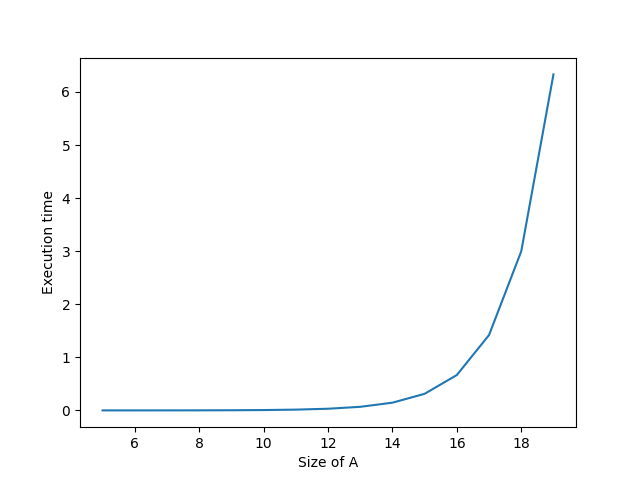
\includegraphics[width=0.8\linewidth]{figs/dyn-hard.png}
	\caption{Čas izvajanja algoritma dinamičnega programiranja za slabe instance}
	\label{fig:dyn}
\end{figure}

\subsection{Izčrpno preiskovanje}

Izčrpno preiskovanje z nekaj rezanja bo preiskoval prostor rešitev v širino -
drevo vseh možnih rešitev je shranjeno kot seznam. Iz seznama odstranimo
podvojene elemente in elemente, ki so že presegli $k$, saj vemo, da ne
predstavljajo rešitev.

Algoritem bo najslabše deloval takrat, ko bo $k$ dovolj velik, da se iz seznama
ne bo odstranil noben element. Na ta način bomo preiskali celoten prostor
rešitev, ki je velik $O(2^n)$. $k$ mora tako biti večji od vsote vseh elementov
v množici $A$. Poskrbeti moramo tudi, da se sešteti elementi med seboj ne
podvajajo.

Primera instanc:
\begin{itemize}
	\item $A = \{ 1, 3, 6, 2, 13 \}$, $k = 25$,
	\item $A = \{ 1, 2, 2^2, 2^3 ..., 2^{n-1}, 2^n \}$, $k = 2^{n+1}$. Izvajanje
	algoritma z različnimi velikosti $n$ prikazuje slika \ref{fig:exh}.
\end{itemize}

\begin{figure}
	\centering
	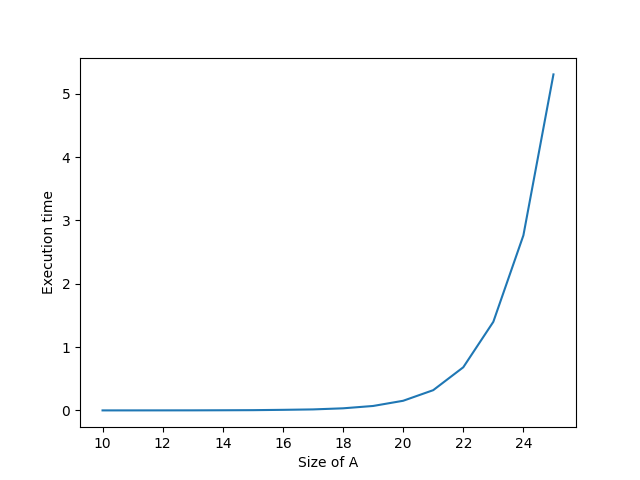
\includegraphics[width=0.8\linewidth]{figs/exh-hard.png}
	\caption{Čas izvajanja algoritma izčrpnega preiskovanja za slabe instance}
	\label{fig:exh}
\end{figure}

\subsection{Požrešni algoritem}

Požrešni algoritem rešitev najde v $O(n \log n)$ času, kjer je $n$ število predmetov. Vemo, da bo najslabša rešitev največ dvakrat slabša od optimalne, kar lahko pokažemo na primeru $A = \{(M + 1), M, M \}, k = 2M$, kjer bomo dobili rešitev $(M+1)$. V splošnem mora veljati $\max\{A\} < k < \max\{A\} + \min\{A\}$. S tem zagotovimo, da bo izbran le največji element iz $A$.

Primera instanc:
\begin{itemize}
	\item $A = \{ 11, 10, 10 \}$, $k = 20$
	\item $A = \{ 11, 9, 10, 12, 13, 14 \}$, $k = 22$
\end{itemize}


\subsection{Polinomska aproksimacijska shema}

Algoritem FPTAS je lahko poljubno natančen, kar določa parameter $\epsilon$.


Tako, da trim ne poreže ničesar (dokaj veliki elementi med sabo).

Kako narediti največjo napako -> če jih je veliko trimmanih.


\begin{figure}
	\centering
	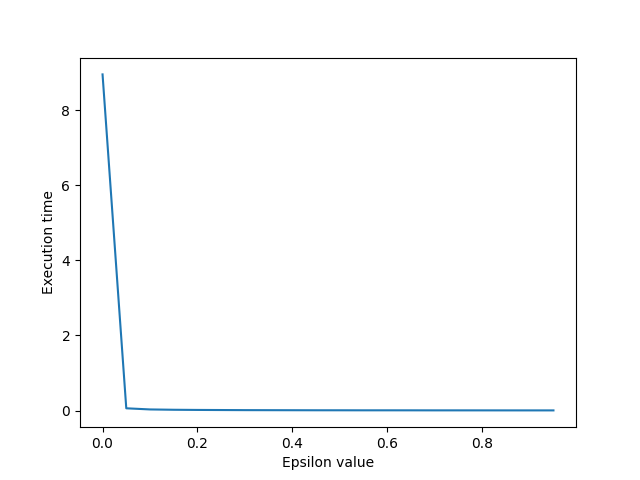
\includegraphics[width=0.8\linewidth]{figs/ss4.png}
	\caption{Čas izvajanja algoritma FPTAS v odvisnosti od $\epsilon$ za primer SS4}
	\label{fig:ss4}
\end{figure}

\begin{figure}
	\centering
	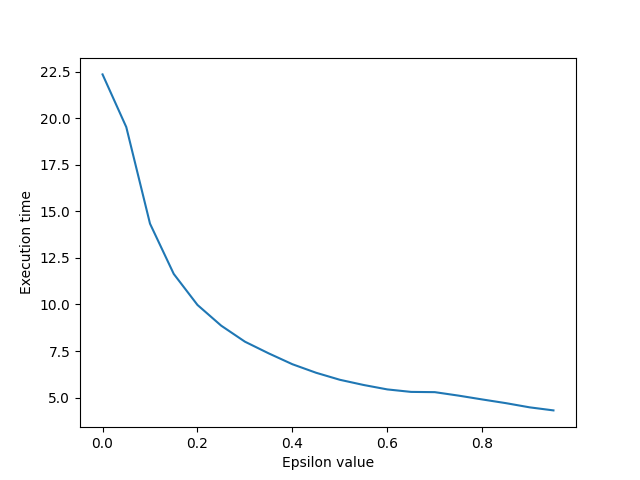
\includegraphics[width=0.8\linewidth]{figs/ss5.png}
	\caption{Čas izvajanja algoritma FPTAS v odvisnosti od $\epsilon$ za primer SS5}
	\label{fig:ss5}
\end{figure}


\end{document}